\documentclass[tikz,border=3pt]{standalone}
\usepackage[T1]{fontenc}
\usepackage{lmodern}
\usepackage{xcolor}
\usetikzlibrary{arrows.meta,positioning}

\definecolor{wine}{HTML}{8A2636}
\definecolor{softblue}{HTML}{EAF2F8}
\definecolor{softgray}{HTML}{F1F2F4}
\definecolor{ink}{HTML}{25282D}

\begin{document}
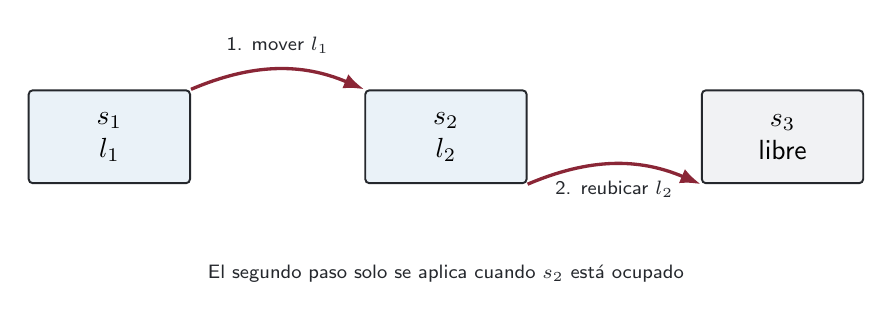
\begin{tikzpicture}[
  font=\sffamily,
  slot/.style={draw=ink, rounded corners=1.5pt, minimum width=2.05cm, minimum height=1.18cm, align=center, line width=0.7pt},
  move/.style={-{Latex[length=2.6mm]}, line width=1.2pt, draw=wine},
  note/.style={font=\sffamily\scriptsize, text=ink, align=center}
]
  \node[slot, fill=softblue] (s1) {\textbf{$s_1$}\\$l_1$};
  \node[slot, fill=softblue, right=2.2cm of s1] (s2) {\textbf{$s_2$}\\$l_2$};
  \node[slot, fill=softgray, right=2.2cm of s2] (s3) {\textbf{$s_3$}\\libre};

  \draw[move, bend left=23] (s1.north east) to node[note, above=2pt] {1. mover $l_1$} (s2.north west);
  \draw[move, bend left=23] (s2.south east) to node[note, below=2pt] {2. reubicar $l_2$} (s3.south west);

  \node[note, below=9mm of s2] {El segundo paso solo se aplica cuando $s_2$ está ocupado};
\end{tikzpicture}
\end{document}
